\section{ЗАДАНИЕ}

Используя хвостовую рекурсию, разработать программу, позволяющую найти 

\begin{enumerate}
    \item n!,
    \item n-е число Фибоначчи.
\end{enumerate}

\begin{lstlisting}[caption=Текст программы]
predicates
	factorial(integer, integer).
	fibb(integer, integer).

clauses
	factorial(0, Result) :- Result = 1, !.
	factorial(N, Result) :-
		NextN = N - 1,
		factorial(NextN, NextResult),
		Result = N * NextResult.

	fibb(1, Result) :- Result = 1, !.
	fibb(2, Result) :- Result = 1, !.
	fibb(N, Result) :-
		PN = N - 1, PPN = N - 2,
		fibb(PN, PResult), fibb(PPN, PPResult),
		Result = PResult + PPResult.

goal
	write("5! : "),
	factorial(5, Result);
	write("f(10) : "),
	fibb(10, Result).
\end{lstlisting}

\section{РЕЗУЛЬТАТ РАБОТЫ}

\begin{figure}[H]
    \centering
    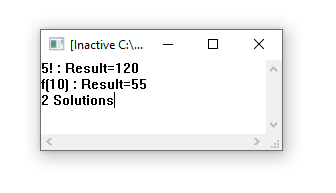
\includegraphics{img/result.png}
    \caption{Результат работы программы}
\end{figure}
